\documentclass[12pt]{article}
\renewcommand{\baselinestretch}{1.15}

\usepackage[utf8]{inputenc} 
\usepackage{lmodern}
\usepackage[T1]{fontenc}
\usepackage{pdfpages}
\usepackage{geometry}
\usepackage[round]{natbib} 
\usepackage[german, american]{babel}
\usepackage{graphicx}
\usepackage{acro}
\usepackage{siunitx}
%\usepackage{hyperref}
\usepackage{setspace}
\usepackage[font={footnotesize}]{caption}


\setlength{\parskip}{0.45em}

\acsetup{first-style=short}
\geometry{
a4paper,
total={170mm,245mm},
left=27mm,
top=20mm,
right =20mm
}


\begin{document}
\pagenumbering{gobble}

\textbf{title:} 'TriangleMethod: An R package to estimate actual evapotranspiration patterns from remote sensing imagery'

\textbf{tags:}
- R
- evaoptranspiration
- landsat
- remote sensing

\textbf{authors:}


- name: David Gampe, 
orcid: 0000-0003-2493-7036,
affiliation: 1


- name: Verena Huber García,
affiliation: 1


- name: Philip Marzahn,
affiliation: 2

- name: Benjamin Müller,
affiliation: 1


\textbf{affiliations:}
- name: Department of Geography, Ludwig-Maximilians-Universität, Munich,
index: 1


- name: Agrar- und Umweltwissenschaftliche Fakultät, Universität Rostock,
index: 2

\textbf{date: 22 October 2021}, bibliography: paper.bib

\section*{ Summary}

Actual evapotranspiration represents one of the most important variables of the hydrological cycle. However, evapotranspiration is characterized by strong temporal and spatial variability. Local observations fail to describe the spatial patterns of evapotranspiration at a regional scale. Furthermore, spatially explicit information of evapotranspiration are not readily available in high resolution and for all areas of the globe. The accurate estimation of evapotranspiration is nevertheless crucial for agricultural and water management purposes as well as to understand interactions between the land surface and the atmosphere. This becomes even more crucial in regions experiencing water scarcity, such as the Mediterranean. Here, the natural water balance is likely altered by irrigation while spatially explicit information on irrigation quantities are usually not available. 

The estimation of actual evapotranspiration through the Triangle Method is based on information on active vegetation and surface temperature. This follows the reasoning that evapotranspiration causes cooling of the surface and vegetated surfaces usually evaporate more than e.g. bare soil under comparable conditions \citep{Carlson2007}. The Normalized Difference Vegetation Index (NDVI) provides information on the greenness of the surface and serves as an estimate for vegetation cover in this method. The land surface temperature (LST) is estimated using the radiometric surface temperature, i.e. brightness temperature, of the sensor in the thermal bands. Both steps are implemented in the R package through the functions \textit{ndvi()} and \textit{tstm()} for Landsat TM images and \textit{tsetm()} for ETM+ images. Except for the different calibration parameters, the latter two functions differ in their structure, as ETM+ has two bands in the thermal infrared, TM only has one. While these two sensors are implemented as default due to their availability and high spatial resolution, the functions can also be modified to derive evapotranspiration patterns from other sensors such as drone imagery \citep{Marzahn2020}. The main functions included in the package are summarized in table 1.

\begin{table}[h!]
\begin{center}
\caption{Overview of the main functions of the package 'TriangleMethod'.}
\label{tab:mainfunc}
\begin{tabular}{ l | l }
% \toprule 
\textbf{Function} & \textbf{Calculation} \\
% \midrule 
\textit{ndvi} & NDVI from the provided remote sensing images \\
\textit{tstm} & Radiometric surface / sensor brightness temperature for Landsat TM\\
& or comparable sensors with single band thermal information\\
\textit{tsetm} & Radiometric surface / sensor brightness temperature for Landsat ETM+\\
& or comparable sensors with two band thermal information\\
\textit{ndvits.plot} & NDVI-LST plot to estimate dry and wet edge temperatures\\
\textit{triangle} & Calculation of actual evapotranspiration from NDVI and LST\\
\textit{cloud.mask} & Simple algorithm to detect \& mask clouds in remote sensing images\\
% \bottomrule 
\end{tabular}
\end{center}
\end{table}

The estimation of evapotranspiration is thus based on the surface energy balance, where surface latent heat flux \textit{$\lambda$E} , equivalent to actual evapotranspiration, is calculated as follows,

\begin{equation}
\label{eq:en.bal}
\lambda E = R\textsubscript{n} - G - H 
\end{equation}

where \textit{Rn} represents the net radiation, \textit{G} the soil heat flux and \textit{H} the sensible heat flux.

Following \citet{Priestleyetal1972}, the equation is restructured and the Priestley-Taylor coefficient $\Phi$ is introduced to substitute the resistance terms of the Penman evaporation scheme \citep{Penman1956}. Thus, the simplified estimation of \textit{$\lambda$E} following \citet{Priestleyetal1972} can be formulated as

\begin{equation}
\label{eq:phi}
\lambda E = \Phi [(R\textsubscript{n} - G) \frac{\Delta}{(\Delta + \gamma)}]
\end{equation}

with the Priestley-Taylor coefficient \textit{$\Phi$}, the slope of the saturated water vapor pressure \textit{$\Delta$} and the psychrometric constant \textit{$\gamma$}.
The evaporation in each pixel, $\lambda$E, is then estimated based on scaling the Priestley-Taylor coefficient \textit{$\Phi$} applying the evaporative fraction \textit{EF}, as the ratio of evapotranspiration \textit{ET}, and available energy. 
EF is thus derived from scaling of $\Phi$ using the NDVI and LST. Following the general reasoning of evaporative cooling, low EF values are expected over pixels with minimum NDVI and maximum temperature and are thus represented by $\Phi$\textsubscript{Min}. Pixels with the highest NDVI and potentially cooler surface temperature are assigned values close to $\Phi$\textsubscript{Max}. The necessary calculation steps can be summarized as follows:

\begin{enumerate}
\item Calculation of NDVI and radiometric surface temperature.
\item Defining the temperature borders through the NDVI-Temperature space.
\item Scaling of $\Phi$ and calculation of evapotranspiration based on EF.
\end{enumerate}

When the NDVI values of a scene are contrasted in a scatter plot to the calculated LST values, most pixels are arranged in a way that they form a triangle \citep{Carlson2007}, giving the name of the method. Negative NDVI values are attributed to water pixels. A general assumption is that the pixels represent the full range of surfaces from densely covered vegetation to bare soil \citep{Carlson2007}. Based on the NDVI-LST scatterplot, the wet and dry edge must be set for each scene. They form the borders of the triangle and are interpreted as physically limiting conditions for evapotranspiration \citep{Batraetal2006} and have to be assigned to derive the final evapotranspiration. The heterogeneity in the scatterplot is attributed to various land covers and the effect of evaporative cooling, which in turn depends on the soil moisture availability \citep{Stisenetal2008}. The more water can evaporate, the more a surface is cooled. Thus, pixels with lowest LST values are the wettest ones and show actual evapotranspiration close to potential evapotranspiration. When applying the Triangle Method, the wet or cold edge (blue line in figure 1) represents the temperature where potential evapotranspiration occurs. 

\begin{figure}[htbp]
\centering
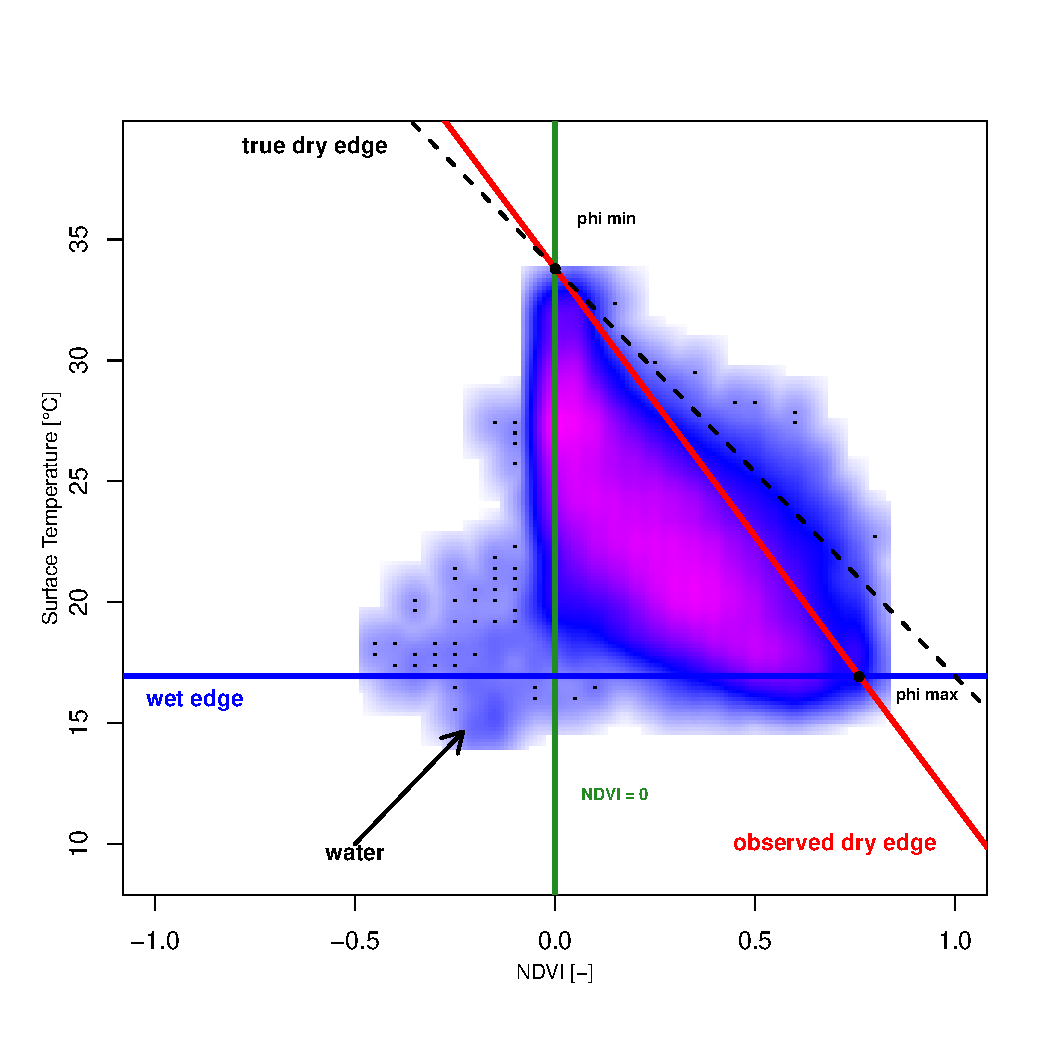
\includegraphics[width=1\linewidth]{NDVI-LST-plot} 
\caption{Resulting NDVI-LST plot to scale the dry and wet edge temperatures for the sample scene.}
\label{figure:ndvilstplot}
\end{figure}



\section*{Statement of need}

Due to these limitations, several studies have been carried out to estimate the spatial distribution of actual evapotranspiration. Remote sensing imagery allows to provide estimates for actual evapotranspiration on a larger scale. As hydrological studies are often carried out in data scarce regions \citep{Gampeetal2016, Meyeretal2016}, it is a prerequisite to depend on as little additional data as possible to derive the patterns of actual evapotranspiration. These requirements are met by the so called 'Triangle Method', originally presented by \citet{Jiangetal1999}. The method uses the Normalized Difference Vegetation Index (NDVI) and land surface temperature (LST) to scale the evaporation fraction (EF) of each pixel. The package allows for simple processing of a multitude of remote sensing images and includes all functions to calculate the necessary inputs from the original remote sensing data. The default sensor in the package is Landsat TM. However, this can easily be adapted for other sensors that provide the required spectral information through the calibration parameter files of the sensor. The Triangle Method has been applied in numerous studies \citep{Batraetal2006, Gampe2016, Stisenetal2008, Tangetal2010, Yangetal2011} and yielding good agreement with deviations from point-measurements of 10 - 30 \% \citep{Kalmaetal2008}. However, a standardized approach of the Triangle Method is still lacking as the studies differ in various calculation steps and in their assumptions. Further, a detailed comprehensive workflow to derive evapotranspiration patterns from raw remote sensing imagery is missing. Consequently, the application of the method requires an enormous effort to collect the necessary information and compile the resulting algorithms. This R-package bridges this gap as it allows the user to apply the Triangle Method with a minimum of essential ancillary information. As further all calculation steps of the aforementioned studies are implemented in the package, the user can compare the different approaches. The package facilitates the calculation process, represents the most important studies where the method has been applied and thus is of great use for future hydrological and ecological studies, particularly in data scarce regions. 

\bibliography{paper}
\bibliographystyle{apalike}

\end{document}
